\documentclass{article}

\usepackage{graphicx}
\usepackage{tikz}
\usepackage{tikzsymbols}
\usetikzlibrary{calc,patterns,shapes.geometric}
\pagestyle{empty}
\usepackage[margin=0pt]{geometry}
\geometry{papersize={14in,12in}}

\def\centerarc[#1](#2)(#3:#4:#5){\draw[#1] ($(#2)+({#5*cos(#3)},{#5*sin(#3)})$) arc (#3:#4:#5);}

\begin{document}
	\begin{figure}
		\centering
		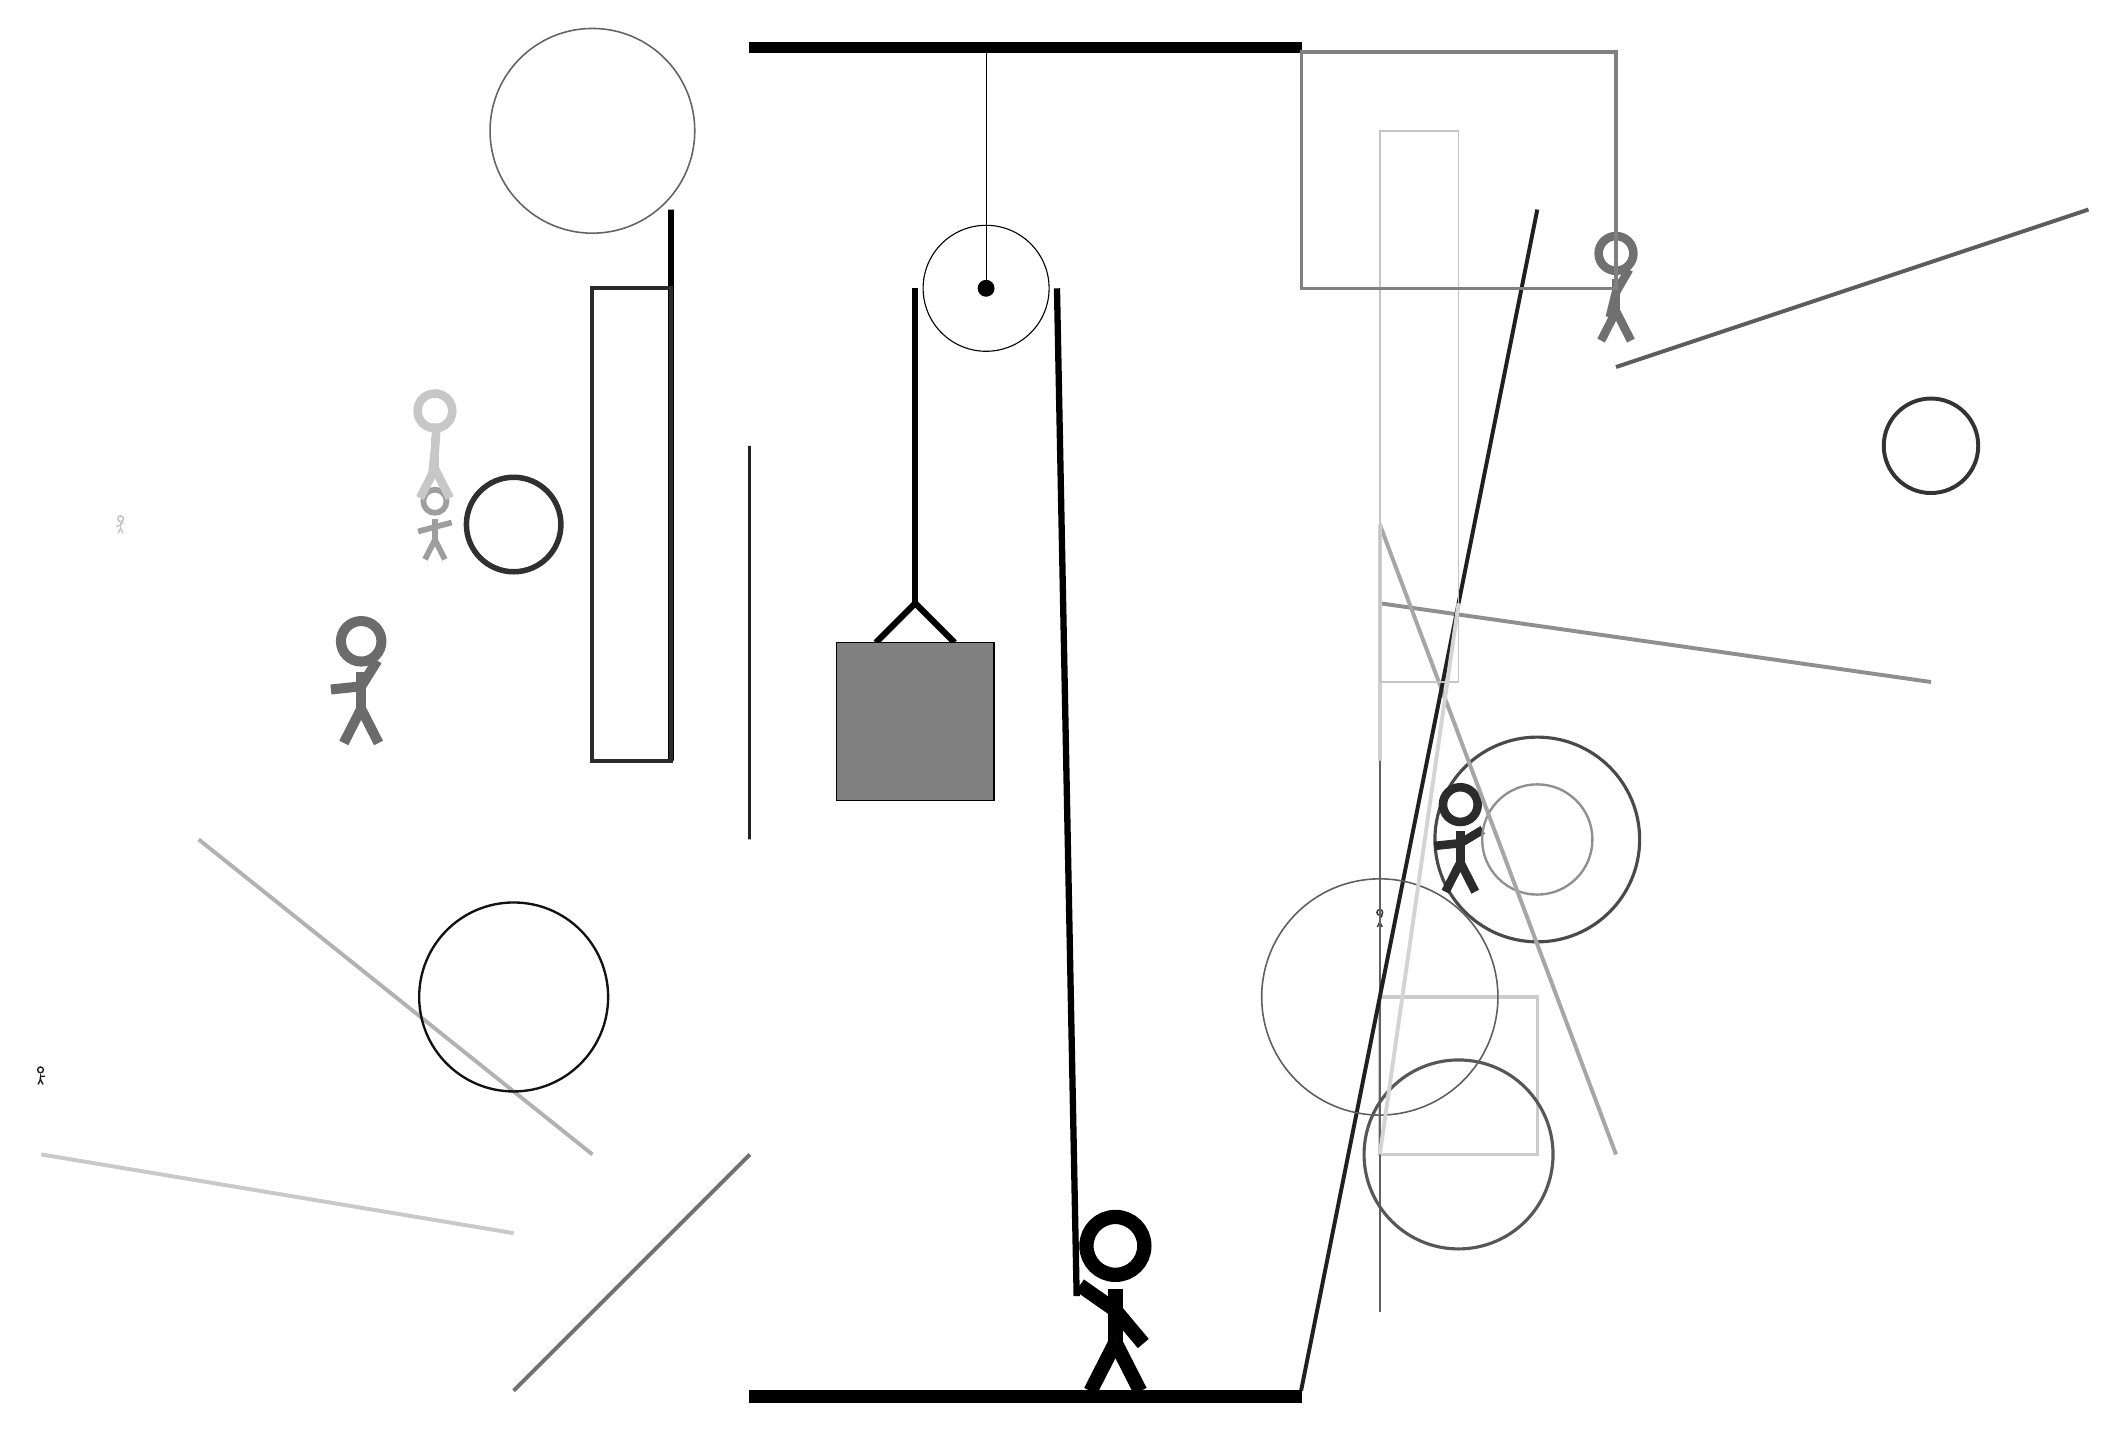
\begin{tikzpicture}
			%%%%% START %%%%%
			
			\draw[fill=black] (-2, 14) rectangle (5, 14.125);
			
			\draw[line width=0.5mm, color=black!30](-4, 0) -- (-9, 4);
			
			\draw[line width=0.4mm, color=black!87] (-2, 4) rectangle (-2, 9);
			\node[line width=0.2mm, color=black!80] at (6, 3) {\Strichmaxerl[1][88][57]};
			\node[line width=0.3mm, color=black!38] at (-6, 8) {\Strichmaxerl[4][15][15]};
			\draw[line width=0.5mm, color=black!64](9, 10) -- (15, 12);
			\node[line width=0.6mm, color=black!56] at (9, 11) {\Strichmaxerl[6][76][60]};
			
			\draw[line width=0.5mm, color=black!56](-5, -3) -- (-2, 0);
			
			\draw [line width=0.5mm, color=black!80](13, 9) circle (0.6);
			\draw[line width=0.7mm, color=black!100] (-3, 12) rectangle (-3, 5);
			\draw [line width=0.4mm, color=black!71](8, 4) circle (1.3);
			\node[line width=0.5mm, color=black!83] at (7, 4) {\Strichmaxerl[6][6][31]};
			\draw[line width=0.5mm, color=black!44](6, 7) -- (13, 6);
			\draw [line width=0.3mm, color=black!44](8, 4) circle (0.7);
			
			\draw [line width=0.3mm, color=black!93](-5, 2) circle (1.2);
			\node[line width=0.5mm, color=black!24] at (-10, 8) {\Strichmaxerl[1][18][53]};
			\draw [line width=0.2mm, color=black!61](-4, 13) circle (1.3);
			
			\draw[line width=0.5mm, color=black!35](6, 8) -- (9, 0);
			\draw[line width=0.5mm, color=black!18] (6, 5) rectangle (6, 8);
			\draw[line width=0.4mm, color=black!20] (6, 2) rectangle (8, 0);
			\draw[line width=0.2mm, color=black!62] (6, -2) rectangle (6, 5);
			\node[line width=0.2mm, color=black!88] at (-11, 1) {\Strichmaxerl[1][88][1]};
			\draw [line width=0.4mm, color=black!66](7, 0) circle (1.2);
			\draw[line width=0.5mm, color=black!88](8, 12) -- (5, -3);
			\draw[line width=0.5mm, color=black!83] (-4, 5) rectangle (-3, 11);
			\draw [line width=0.2mm, color=black!63](6, 2) circle (1.5);
			\draw [line width=0.7mm, color=black!81](-5, 8) circle (0.6);
			\draw[line width=0.5mm, color=black!21](-5, -1) -- (-11, 0);
			\node[line width=0.3mm, color=black!22] at (-6, 9) {\Strichmaxerl[6][84][86]};
			
			\draw[line width=0.2mm, color=black!23] (6, 13) rectangle (7, 6);
			
			\draw[line width=0.5mm, color=black!17](7, 7) -- (6, 0);
			\node[line width=0.7mm, color=black!58] at (-7, 6) {\Strichmaxerl[7][6][58]};
			
			\draw[line width=0.4mm, color=black!50] (5, 11) rectangle (9, 14);
			
			\draw (1, 11) circle (0.8);
			\draw[fill=black] (1, 11) circle (0.1);
			\draw (1, 14) -- (1, 11);
			
			\draw[line width=0.8mm] (-0.4, 6.5) -- (0.1, 7.0) -- (0.6, 6.5);
			\draw[fill=black!50] (-0.9, 6.5) rectangle (1.1, 4.5);
			
			\draw[line width=0.8mm] (0.1, 11) -- (0.1, 7.0);
			\centerarc[line width=0.8mm](1, 11)(0:180:0.9);
			\draw[line width=0.8mm](1.9, 11) -- (2.15, -1.8);
			
			\node at (2.6, -1.9) {\Strichmaxerl[10][-35][-50]};
			
			\draw[fill=black] (-2, -3) rectangle (5, -3.15);
			
			%%%%% END %%%%%
		\end{tikzpicture}
	\end{figure}	
\end{document}